\documentclass{article}
\title{Sistema de controle de mesa de som - Sistemas digitais e microcontrolados}
\date{}

\usepackage[utf8]{inputenc}
\usepackage[portuguese]{babel}
\usepackage[margin=3.5cm]{geometry}
\usepackage{amsmath}
\usepackage{physics}
\usepackage{titlesec}
\usepackage{graphicx}
\usepackage{wrapfig}
\usepackage{caption}
\usepackage{subcaption}
\usepackage{karnaugh-map}
\usepackage[parfill]{parskip}
\usepackage[nottoc]{tocbibind}
\usepackage[backend=biber]{biblatex}
\addbibresource{/home/luispengler/drive/LinuxFabrik/Research/read/bib.bib}
\usepackage{authblk}
\author[1]{Giovanna Bughi}
\author[2]{Gustavo Ratier Cardoso}
\author[3]{João Vitor Medeiros}
\author[4]{Luís Spengler}
\affil[1,2,3,4]{Instituto Federal de Educação, Ciência e Tecnologia de Mato Grosso do Sul}

\graphicspath{{./docs/}}

\begin{document}
\maketitle

\tableofcontents

\medskip

\section{Problema proposto}
Uma mesa de som conecta três microfones numa única caixa de som amplificada, que são: Microfone Presidente, Microfone Diretor e Microfone Coordenador. Sabendo que somente um microfone pode falar por vez. Elabore um circuito lógico combinacional que permita ligar os microfones segundo a prioridade abaixo:

Prioridade 1 : Presidente         

Prioridade 2 : Diretor

Prioridade 3 : Coordenador

Cada Microfone é acionado pelo usuário por um interruptor  ( liga-desliga) (ChP, ChD, ChC). Cada microfone  ao ser acionado tem sua saída  comutada (0 ou 1) informando ao circuito lógico,  que por sua vez, aciona uma das  saídas (SP, SD, SC), para a caixa amplificada. Então, quando o Presidente ligar seu microfone, terá prioridade sobre os demais. Quando o Diretor ligar seu microfone só terá prioridade sobre o  Coordenador. O Coordenador só fala quando os demais não estiverem com seus microfones ligados.

\subsection{Esboço do esquema proposto}
O problema pode ser esboçado de acordo com o texto apresentado acima.

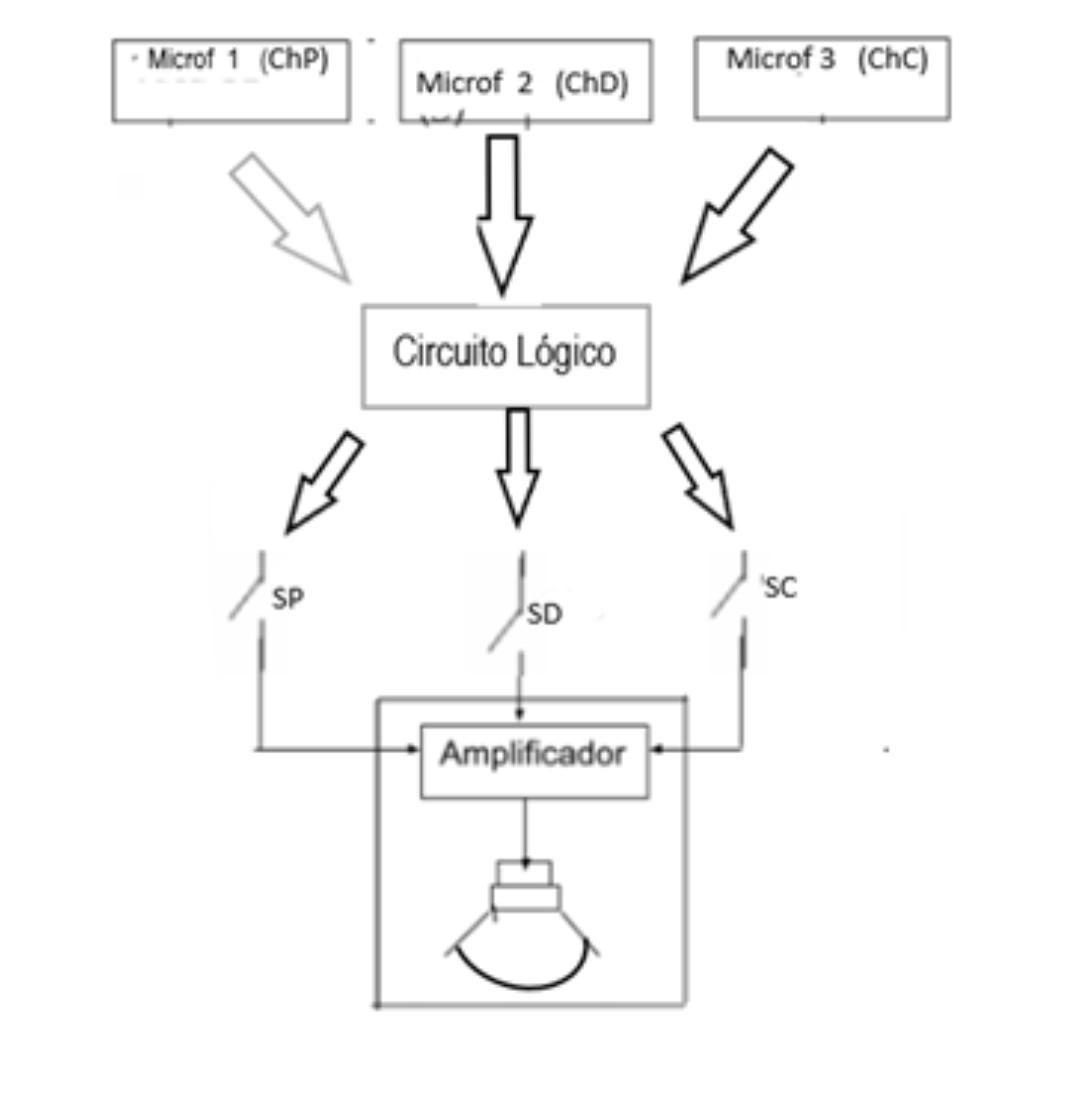
\includegraphics[width=\textwidth]{esbocoroubado}

\section{Solução do problema proposto}

\subsection{Identificação das variáveis de entrada e saída}
Foi definido a cada usuário do microfone uma variável distinta, estas sendo as variáveis de entrada (ChP, ChD, ChC). Foram definidas como variáveis de saída SP, SD e SC, suas respectivas saídas.

\subsection{Identificação dos estados das variáveis de entrada e saída}
As entradas (ChP, ChD, ChC) apenas serão 1 (nível lógico alto) quando os usuários tiverem seus microfones ligados. Se todos tiverem seus microfones ligados, então ChP=1, ChD=1, ChC=1. No entanto, em um estado inicial, todas as variáveis serão igual a 0, portanto: ChP=0, ChD=0, ChC=0. Conforme a conversa prossegue, cada um dos usuários (que aqui são as variáveis de entrada), alterarão o seu estado lógico para o nível 1.

\subsection{Montagem da tabela verdade}
 Obedecendo a prioridade de cada falante, as saídas na tabela verdade podem ter seus estados definidos pelos valores abaixo.
\begin{displaymath}
\begin{array}{|c c c|c c c|}
INPUT & & & OUTPUT &\\
\hline
ChP & ChD & ChC & SP & SD & SC\\
\hline % Put a horizontal line between the table header and the rest.
0 & 0 & 0 & 0 & 0 & 0\\
0 & 0 & 1 & 0 & 0 & 1\\
0 & 1 & 0 & 0 & 1 & 0\\
0 & 1 & 1 & 0 & 1 & 0\\
1 & 0 & 0 & 1 & 0 & 0\\
1 & 0 & 1 & 1 & 0 & 0\\
1 & 1 & 0 & 1 & 0 & 0\\
1 & 1 & 1 & 1 & 0 & 0\\
\end{array}
\end{displaymath}

\subsection{Obtenção da expressão de saída}
A partir da tabela verdade, pôde-se obter as seguintes expressões:
\begin{enumerate}
	\item Para SP, em função de ChP:
		\[SP=ChP\cdot ChC' + ChP\cdot ChC\]
		\[SP=ChP\cdot (ChC' + ChC)\]
		\[SP=ChP\]
	\item Para SD, em função de ChD:
		\[SD=ChP'\cdot ChD\]
	\item Para SC, em função de ChC:
		\[SC=(ChP'\cdot ChD')\cdot ChC\]
\end{enumerate}

\subsection{Mapa de Karnaugh}
Mapa de Karnaugh para a saída do presidente (SP)

\begin{karnaugh-map}*[4][2][1][$ChPChD$][$ChC$]
	\minterms{2,3,6,7}
	\maxterms{0,1,4,5}
	\indeterminants{2,5}
	\implicant{3}{2}
	\implicant{7}{6}
\end{karnaugh-map}

Mapa de Karnaugh para a saída do diretor (SD)

\begin{karnaugh-map}*[4][2][1][$ChPChD$][$ChC$]
	\maxterms{0,2,3,4,6,7}
	\minterms{1,5}
	\implicant{1}{5}
\end{karnaugh-map}

Mapa de Karnaugh para a saída do coordenador (SC)

\begin{karnaugh-map}*[4][2][1][$ChPChD$][$ChC$]
	\maxterms{0,1,2,3,5,6,7}
	\minterms{4}
	\implicant{4}{4}
\end{karnaugh-map}

\subsection{Simplificação da expressão pelo mapa de Karnaugh}
A única expressão que pôde ser simplificada através do mapa de Karnaugh é a expressão referente à SP em função de ChP, pois apenas esta apresenta uma propriedade de simplificação.

\begin{karnaugh-map}*[4][2][1][$ChPChD$][$ChC$]
	\minterms{2,3,6,7}
	\maxterms{0,1,4,5}
	\indeterminants{2,5}
	\implicant{3}{2}
	\implicant{7}{6}
\end{karnaugh-map}

\subsection{Obtenção do circuito lógico}

\subsection{Implementação do hardware a partir do circuito lógico}

\section{Conclusão}

\medskip

\end{document}
